\documentclass{article}
\usepackage{amsmath}
\usepackage{pgfplots}
\pgfplotsset{compat=1.17}
\begin{document}

\title{Electricity and Magnetism - Lecture 8 Notes}
\author{Joshua Clement}
\maketitle

\section*{Review of Potential Energy}
\begin{itemize}
    \item \textbf{Potential Energy} (\(U\)): Energy due to the interaction between charges.
    \item \textbf{Interaction Energy}: Comes from the interaction of two or more charges.
    \item \textbf{Internal Work}: Work done within a system to move charges from one position to another.
    \[
        \Delta U = -W_{\text{internal}}
    \]
    \item Another way for a uniform field in the x-direction:
    \[
        \Delta U = -qE \Delta x
    \]
\end{itemize}

\section*{Electric Potential Energy}
\begin{itemize}
    \item \textbf{Electric Potential Energy} (\(U_{\text{el}}\)): The work required to bring a charge from infinity to a specific position in the presence of other charges.
    \[
    U_{\text{el}} = \frac{1}{4 \pi \epsilon_0} \frac{q_1 q_2}{r}
    \]
    where \(q_1\) and \(q_2\) are charges and \(r\) is the distance between them.
    \item \textbf{Like Charges} (\(q_1, q_2 > 0\)): \(U_{\text{el}} > 0\), indicating repulsion.
    \item \textbf{Opposite Charges} (\(q_1, q_2 < 0\)): \(U_{\text{el}} < 0\), indicating attraction.
\end{itemize}

\section*{Electric Potential}
\begin{figure}[h!]
    \centering
    % Positive Charge Plot
    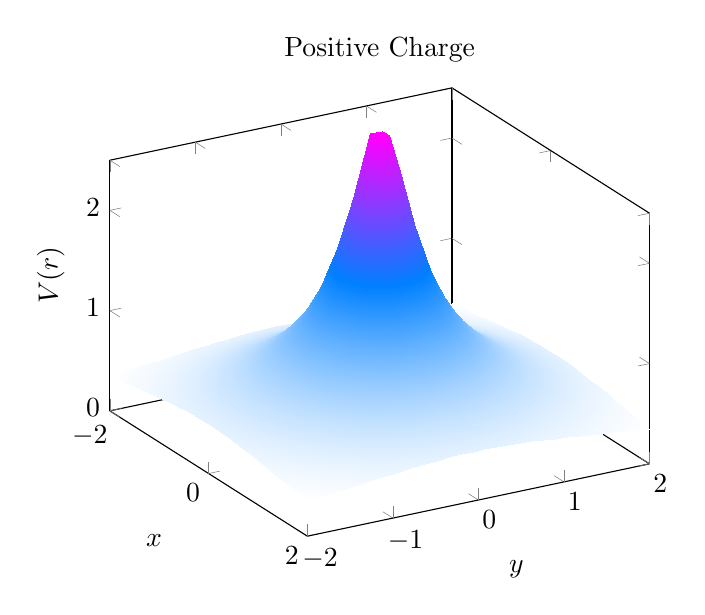
\begin{tikzpicture}
        \begin{axis}[
            view={60}{30},
            xlabel={$x$},
            ylabel={$y$},
            zlabel={$V(r)$},
            domain=-2:2,
            y domain=-2:2,
            colormap/cool,
            samples=30,
            samples y=30,
            zmax=2.5,
            zmin=0,
            mesh/ordering=y varies,
            title={Positive Charge}
        ]
            \addplot3[
                surf,
                shader=interp,
                domain=-2:2,
                y domain=-2:2,
                ]
                {1/sqrt(x^2 + y^2 + 0.1)};
        \end{axis}
    \end{tikzpicture}

    % Negative Charge Plot
    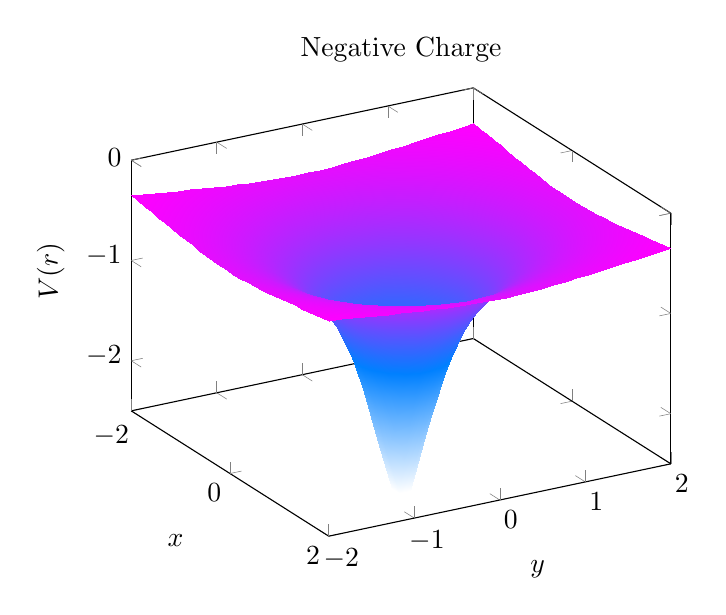
\begin{tikzpicture}
        \begin{axis}[
            view={60}{30},
            xlabel={$x$},
            ylabel={$y$},
            zlabel={$V(r)$},
            domain=-2:2,
            y domain=-2:2,
            colormap/cool,
            samples=30,
            samples y=30,
            zmax=0,
            zmin=-2.5,
            mesh/ordering=y varies,
            title={Negative Charge}
        ]
            \addplot3[
                surf,
                shader=interp,
                domain=-2:2,
                y domain=-2:2,
                ]
                {-1/sqrt(x^2 + y^2 + 0.1)};
        \end{axis}
    \end{tikzpicture}

    \caption{Electric potential (\(V(r)\)) as a scalar field for a positive (left) and negative (right) charge.}
    \label{fig:potential_scalar_field}
\end{figure}

\begin{itemize}
    \item \textbf{Electric Potential} (\(V\)): The potential to have electric potential energy if a test charge is introduced.
    \item \textbf{Electric Potential Due to a Point Charge}:
    \[
    V(r) = \frac{1}{4 \pi \epsilon_0} \frac{q}{r}
    \]
    where \(q\) is the source charge and \(r\) is the distance from the charge.
    \item \textbf{Units}: The unit of electric potential is \textbf{Volts (V)}.
    \item \textbf{Equipotential Surfaces}: Surfaces where the electric potential is constant; for a point charge, these surfaces are spherical.
\end{itemize}

\section*{Electric Potential Difference}
\begin{itemize}
    \item \textbf{Electric Potential Difference in a Nonuniform E-Field} (\(\Delta V)\)):
    \[
        \Delta V = V_B - V_A = -\int_i^f \vec{E} \cdot d\vec{l}
    \]
    \item \textbf{Potential Difference} (\(\Delta V\)): The difference in electric potential between two points.
    \[
    \Delta V = V_B - V_A = -E \Delta x
    \]
    where \(E\) is the electric field and \(\Delta x\) is the displacement in the direction of the field.
    \item \textbf{Relation to Work}: The work done by the electric field in moving a charge \(q\) between two points is:
    \[
    W = q \Delta V
    \]
\end{itemize}

\section*{Electric Potential Energy of Multiple Charges}
\begin{itemize}
    \item \textbf{System of Charges}: The total electric potential energy is the sum of the interaction energies between all pairs of charges.
    \[
    U_{\text{sys}} = \sum_{i<j} \frac{1}{4 \pi \epsilon_0} \frac{q_i q_j}{r_{ij}}
    \]
    \item \textbf{Adding a New Charge} (\(q_3\)): The work needed to bring a new charge \(q_3\) from infinity to point \(C\) is given by:
    \[
    U_{\text{sys}} = U_{12} + V_C q_3
    \]
    where \(V_C\) is the electric potential at point \(C\) due to the other charges.
\end{itemize}

\section*{Electron-Volt (eV)}
\begin{itemize}
    \item \textbf{Electron-Volt (eV)}: The energy required to move a charge of \(1e\) through a potential difference of \(1V\).
    \[
    1 \text{ eV} = 1.6 \times 10^{-19} \text{ J}
    \]
    \item \textbf{Example}: If a proton moves in an electric field and loses \(1 \text{ eV}\) of potential energy, its kinetic energy increases by \(1 \text{ eV}\).
\end{itemize}

\section*{Electric Potential as a Scalar Field}
\begin{itemize}
    \item \textbf{Scalar Field}: The electric potential is a scalar quantity and can be represented as a field in space.
    \item \textbf{Superposition Principle}: The total electric potential at a point is the sum of the potentials due to individual charges.
    \[
    V_P = \frac{1}{4 \pi \epsilon_0} \left( \frac{q_1}{r_1} + \frac{q_2}{r_2} \right)
    \]
    \item \textbf{Equipotential Surfaces}: For a point charge, these surfaces are spherical and indicate regions with the same potential.
\end{itemize}

\end{document}